% !TEX root = proposal.tex
\chapter{Conflict Resolution}
\label{sec:conflicts}

Conflicts arise naturally in a participatory network, as \sys is
designed to allow multiple, distributed principals to author the network configuration.
For example, one principal may issue a request to deny traffic to
TCP port 80, while another may request  such traffic be allowed.
This chapter discusses how \sys handles conflicts between overlapping requests
through the introduction of Hierarchical Flow Tables (HFTs).

Two requests overlap when the intersection of their
respective flowgroups is not empty, \ie, there are some flows that
match both.  As described in \xref{sec:overview}, principals
make requests in the context of a share, and accepted requests
become policy atoms residing in this share. Policy atoms, then,
inherit from the share tree a natural hierarchical relationship,
which we call the \emph{policy tree}. The network's effective policy is a function
of the set of all policy atoms, their position in the tree, and the
semantics of conflict resolution between overlapping policy atoms.

We now develop a detailed semantics for HFTs (\xref{sec:Implementation}),
describe a compiler which translates HFTs for use in OpenFlow-based SDNs (\label{s:lin}), 
detail \sys's choice of conflict-resolution operators (\xref{sec:conflict-resolution-operators}),
the fulfillment of \emph{strict} and \emph{partial} requests, (\xref{sec:strict-partial}),
and finally, analyze the complexity of the \treelang compiler (\xref{sec:compiler-complexity}).

\section{Semantics of \treelang}
\label{sec:Implementation}

A Hierarchical Flow Table allows several principals to author a tree of policies, and
specify custom conflict-resolution operators at each node in the
tree. In this section, we define the semantics of a policy tree as the
final action it produces on an individual packet, after it has
consolidated actions from all policies in the tree.\footnote{This
  semantic model, where the central controller conceptually sees all
  packets, is inspired by Frenetic~\cite{Foster:2010}.}
In \xref{s:lin}, we compile these policy trees to run efficiently on hardware.
%Because our switches cannot directly implement these trees, thus in section~\ref{s:lin},
%we linearize these trees to \emph{network flow tables}, which
%are easy to use in our runtime to configure switches.
%{\color{red} We conclude with a theorem that this translation is correct.} % where did we put it?

\begin{figure}

\begin{displaymath}
\begin{array}{lrcl}
& H & = & \textrm{header names and ingress ports} \\
\textrm{patterns} & V & = & \textit{const} \mid \textit{prefix} \mid \star \\
\textrm{matches} & M & = & 
  \emptyset \mid \langle \overrightarrow{H,V} \rangle \\
\textrm{actions} & A & = & \textbf{Allow} \mid \textbf{Deny} 
  \mid \textbf{Reserve}(n) \mid \textbf{RateLimit}(n) \mid \textbf{0} \\
\textrm{conflict-resolution} & (+)  & = & A \rightarrow A \rightarrow A \\
\textrm{operators} \\
\textrm{policy atoms} & P & = & M \times A \\
\textrm{policy tree nodes} & D & = & (+_D) \times 2^P \\
\textrm{policy trees} & T & = & (+_P) \times (+_S) \times D \times 2^{T} \\
\textrm{packets} & K & = & \langle \overrightarrow{H,\mathit{const}} \rangle
\end{array}
\end{displaymath}

\fbox{$\mathit{cmb} : D \times K \rightarrow A$}
\begin{displaymath}
\begin{array}{l}
\mathit{cmb}((+,\{ \cdots (M_i,A_i) \cdots \}), K) = 
  A'_1 + \cdots + A'_k + \textbf{0} \\
\begin{array}{lrcl}
\textrm{where} & \{ A'_1, \cdots, A'_k \} & = & \{ A_i | M_i \cap K \ne \emptyset \}
\end{array}
\end{array}
\end{displaymath}

\fbox{$\mathit{eval} : T \times K \rightarrow A$}
\begin{displaymath}
\begin{array}{l}
\textit{eval}((+_P,+_S,D,\{ T_1,\cdots, T_n \}), K) = \textit{cmb}(D, K) +_P A_1 \\
\begin{array}{lrcl}
\textrm{where}
& A_1 & = & eval(T_1,K) +_S A_2 \\
& A_2 & = & eval(T_2,K) +_S A_3 \\
& \cdots \\
& A_n & = & eval(T_n,K) +_S \textbf{0}
\end{array}
\end{array}
\end{displaymath}

\caption[Caption for Semantics]{Semantics of \treelang \footnotemark }
\label{f:sharesem}
\end{figure}


Figure~\ref{f:sharesem} defines packets ($K$), policy trees ($T$),
actions $(A)$, and a function $\mathit{eval}$ that matches packets
against policy trees and returns an action.  
For our purposes, packets are 
a vector of header names and values; we do not match on packets'
contents. For concreteness, we depict the actions we have implemented in 
our prototype (\xref{sec:FullSystem}): admission control, reserving a guaranteed
minimum bandwidth (GMB), rate-limiting bandwidth, and $\textbf{0}$, a special ``don't care''
action.

A policy tree is a tree of policy nodes ($D$), which contain sets of policy
atoms ($P$). An atom is a match rule and action pair, $(M,A)$. When a
packet matches a policy atom, $M \cap K \ne \emptyset$, the atom produces
its action. The interesting cases occur when a packet matches several
policy atoms with conflicting actions. In these cases, we resolve conflicts
with the conflict-resolution operators ($+$) attached throughout the policy tree.
\footnotetext{$2^{M \times A}$ is the set of all subsets of pairs drawn from $M$ and $A$.}

Policy trees have different types of conflict-resolution operators at several
points in the tree (\ie, $+_D$, $+_P$, $+_S$ in Figure~\ref{f:sharesem}). 
These multiple types allow an HFT to resolve different types of conflicts using
independent logic. For example, conflicts between parent and child nodes
may be resolved differently than conflicts between a single node's internal
policy atoms.
Therefore, the choice of conflict-resolution operators is a key policy decision.
Our prototype network (\xref{sec:FullSystem}) provides two default operators;
developing and evaluating additional operators, such as operators to
support priorities across requests, is left as future work.

The function $\mathit{cmb}$ matches a packet with an individual policy
tree node. If a packet matches several policy atoms,
$\mathit{cmb}$ uses the node's internal conflict-resolution operator, $+_D$,
to combine their actions. The compiler
requires $+_D$ to be associative and have $\textbf{0}$
as its identity.\footnote{That is, we require $a + (b + \textbf{0}) =
  (a + b) + \textbf{0} = a + b$.}

The function $\mathit{eval}$ matches a packet with a policy tree by
applying $\mathit{cmb}$ to the policy tree node at the root, and
recursively applying $\mathit{eval}$ to its children. A policy tree
has conflict-resolution operators $+_P$ and $+_S$, which respectively allow
it to resolve parent-child and inter-sibling conflicts differently. In
particular, $+_P$ does not have to be commutative -- it is always used
with the parent's action on the left and the child's action on the
right. This lets us express intuitive conflict resolutions such as ``child overrides
parent.''


\begin{figure}
\centering
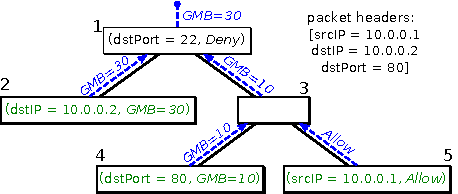
\includegraphics[width=0.7\textwidth]{figs/evaltree}
\caption{Evaluation of a single packet}
\label{f:evaltree}
\end{figure}


\vspace{0.5em}\noindent\textbf{Example:\space}
Figure~\ref{f:evaltree} depicts a simple policy tree
and illustrates how $\mathit{eval}$ produces an action, given the 
tree and indicated packet.
Each node contains its policy atoms, and atoms which match the packet are colored
green. The $\mathit{eval}$ function recursively produces an action from
each sub-tree; these actions are the labels on each node's outgoing edge.

In this example, the policy atoms at each leaf match the packet and produce
an action.
Node $3$ receives conflicting actions
from its children, which it resolves with its inter-sibling
conflict-resolution operator:
$\textbf{Reserve}(10)
+_S \textbf{Allow} = \textbf{Reserve}(10)$. Node $3$ has no policy atoms
itself, so it produces the $\textbf{0}$ action. Since $\textbf{0}$ is
the identity of all conflict-resolution operators,
  $\textbf{0} +_P \textbf{Reserve}(10) = \textbf{Reserve}(10)$ is the
resulting action from this sub-tree. 

Finally, Node 1 computes the aggregate action of its children:
$\textbf{Reserve}(30) +_S \textbf{Reserve}(10) = \textbf{Reserve}(\max(30,10))$.
Since Node 1's policy atoms do not match the packet,
the final action is
$\textbf{0} +_P \textbf{Reserve}(30) = \textbf{Reserve}(30)$.


\section{Compiling Policies}\label{s:lin}

The preceding section assumes that a central function,
$\mathit{eval}$, observes and directs all packets in the network.
Although $\mathit{eval}$ specifies the meaning of policy trees, this is not a
practical implementation. We now describe how to compile \treelang's
policy trees to run on commodity switches, which support simpler, linear
flow tables, to produce a practical implementation.

Our compiler works in two stages. First, we translate policy trees to
\emph{network flow tables}, which have a basic,
linear matching semantics. Second, we use
network flow tables to configure a distributed network of switches,
translating high-level actions such as $\textbf{GMB}(n)$ to low-level
operations on switches (\xref{sec:NIB}).

\begin{figure}[t]

\begin{displaymath}
\begin{array}{lrcl}
\textrm{Network Flow Tables} & N & = & \langle \overrightarrow{M,A} \rangle
\end{array}
\end{displaymath}

\fbox{$\mathit{scan} : N \times K \rightarrow A$}

\medskip

\inference
{M_1\cap K = \emptyset \cdots M_{j-1} \cap K = \emptyset \qquad
 M_j\cap K \ne \emptyset }
{\mathit{scan}(\langle(M_1,A_1)\cdots(M_n,A_n)\rangle,K) = A_j}

\medskip

\inference
{M_1\cap K = \emptyset \cdots M_{n} \cap K = \emptyset}
{\mathit{scan}(\langle(M_1,A_1)\cdots(M_n,A_n)\rangle,K) = \textbf{0}}


\medskip

\fbox{$\mathit{lin}_D : D \rightarrow N$}
\begin{displaymath}
\begin{array}{l}
\mathit{lin}_D\left(+_D,\{M_1,A_1, \cdots, M_j,A_j \}\right) 
  = N_1 \\
\begin{array}{lllll}
\textrm{where} 
& N_1 = \mathit{union}(+_D,\langle M_1,A_1\rangle, N_2) \\
& \cdots \\
& N_j = \mathit{union}(+_D, \langle M_j,A_j\rangle, \langle\rangle)
\end{array}
\end{array}
\end{displaymath}

\fbox{$\mathit{lin}_T : T \rightarrow N$}
\begin{displaymath}
\begin{array}{l}
\mathit{lin}_T\left(+_P,+_S,D, \{T_1\cdots T_k\}\right)
  = \mathit{union}(+_P,\mathit{lin}_D(D), N_1) \\
\begin{array}{lllll}
\textrm{where} 
& N_1 = \mathit{union}(+_S, \mathit{lin}_T(T_1), N'_2) \\
& \cdots \\
& N_k = \mathit{union}(+_S,\mathit{lin}_T(T_k), \langle \rangle)
\end{array}
\end{array}
\end{displaymath}

\fbox{$\mathit{union},\mathit{inter} : (+) \times N \times N \rightarrow N$}
\begin{displaymath}
\begin{array}{l}
\mathit{union}((+),N_1,N_2) = \mathit{inter}((+),N_1,N_2) N_1 N_2 \\
\mathit{inter}((+),\langle\cdots(M_i,A_i)\cdots\rangle, \langle\cdots(M'_j,A'_j)\cdots\rangle) = \\
\qquad \langle\cdots(M_i \cap M'_j,A_i+A'_j))\cdots\rangle
\end{array}
\end{displaymath}

\caption{Network Flow Tables}
\label{f:intermediate}

\end{figure}

A network flow table ($N$) is a sequence of paired match rules
and actions. The $\mathit{scan}$ function, defined in
Figure~\ref{f:intermediate}, matches packets against network flow
tables and returns the action associated with the first matching rule. If
no rules match the packet, then $\mathit{scan}$ returns $\textbf{0}$.\footnote{The
  $\mathit{scan}$ function is derived from 
  NetCore~\cite{Monsanto:2012}.}

The matching semantics of network flow tables correspond to the
matching semantics of switch flow tables exposed by OpenFlow.  When a
packet matches a switch flow table, only one rule's action applies. If a
packet matches multiple rules, the switch selects the one with the
highest priority.  A rule's index in a network flow table corresponds
to a switch flow table priority, with index $0$ as the highest
priority. Since all rules have distinct indices, a naive
correspondence would give all rules distinct priorities. A more
compact one, which we use, maps a sequence of
non-overlapping network flow table rules to a single priority in a
switch flow table.

The $\mathit{lin}_T$ function is our compiler from policy trees to
network flow tables. It uses $\mathit{lin}_D$ as a helper to compile
policy tree nodes.  The $\mathit{lin}_D$ function translates policy
atoms to singleton network flow tables, and combines them with
$\mathit{union(+,N,N')}$.  $\mathit{Union}$ builds a network flow table that
matches packets in either $N$ or $N'$. Moreover, when a packet
matches both $N$ and $N'$, $\mathit{union}$ computes the intersection
using the $+$ conflict-resolution operator to combine
actions.

Similarly, $\mathit{lin}_T$ recursively builds network flow tables for
its subtrees, and calls $\mathit{lin}_D$ on its root node.  It applies
$\mathit{union}$ to combine the results, using $+_S$ and $+_P$ where
appropriate.


The functions in Figure~\ref{f:intermediate}, $\mathit{lin}_T$,
$\mathit{lin}_D$, $\mathit{union}$, and $\mathit{inter}$ require the
conflict-resolution operators to satisfy the following properties.
\begin{wftree}[Well-formed] 
$T$ is well-formed if:
\begin{itemize}

\item All conflict-resolution operators are associative, and

\item $\textbf{0}$ is the identity of all conflict-resolution operators.
\end{itemize}
\end{wftree}
Proving the compiler correct requires the following key lemma, which
states that all conflict-resolution operators distribute over $\mathit{scan}$.
\begin{unioncommute}
For all $+$, $N_1$, and $N_2$, where $\textbf{0}$ is the identity of $+$,
$\mathit{scan}(\mathit{union}(+,N_1,N_2)) = \mathit{scan}(N_1) +
\mathit{scan}(N_2)$.
\end{unioncommute}
With this, we prove the compiler correct.
\begin{compilercorrect}[Soundness]
For all well-formed policy trees, $T$ and packets, $P$, $\mathit{eval}(T, P) =
\mathit{scan}(\mathit{lin}_T(T), P)$.
\end{compilercorrect}
We mechanize all our definitions and proofs using the Coq proof assistant~\cite{coq}. \qed

\section{Conflict-resolution Operators in \sys}
\label{sec:conflict-resolution-operators}


As discussed previously, HFTs resolve conflicts through the use of conflict resolution operators.
These operators take two conflicting requests as input, and return a single
resolved request. For example, a packet which matches policy atoms from \priv{Reserve}(10)
and \priv{Reserve}(30) may be resolved to the higher guaranteed bandwidth,
\priv{Reserve}(30), as occurs at Node 1 in Figure~\ref{f:evaltree}.

\begin{figure}[t]
\begin{small}
\fbox{$+_P : A \times A \rightarrow A$}
\begin{displaymath}
\begin{array}{lclcl}
\textbf{Deny} & +_P & \textbf{Allow} & = & \textbf{Allow} \\
\textbf{Allow} & +_P & \textbf{Allow} & = & \textbf{Allow} \\
A_P & +_P & \textbf{Deny} & = & \textbf{Deny} \\
\textbf{Deny} & +_P & \textbf{Reserve}(n) & = & \textbf{Reserve}(n) \\
\textbf{Reserve}(m) & +_P & \textbf{Reserve}(n) & = & \textbf{Reserve}(\max(m,n)) \\
\textbf{Reserve}(m) & +_P & \textbf{Allow} & = & \textbf{Reserve}(m) \\
\textbf{Allow} & +_P & \textbf{Reserve}(m) & = & \textbf{Reserve}(n) \\
\textbf{Deny} & +_P & \textbf{Ratelimit}(n) & = & \textbf{Ratelimit}(n) \\
\textbf{Ratelimit}(m) & +_P & \textbf{Ratelimit}(n) & = & \textbf{Ratelimit}(\min(m,n)) \\
\textbf{Ratelimit}(m) & +_P & \textbf{Allow} & = & \textbf{Ratelimit}(m) \\
\textbf{Allow} & +_P & \textbf{Ratelimit}(m) & = & \textbf{Ratelimit}(n) \\
\end{array}
\end{displaymath}

\fbox{$+_S : A \times A \rightarrow A$}
\begin{displaymath}
\begin{array}{lclcl}
\textbf{Deny} & +_S & A_2 & = & \textbf{Deny} \\
\textbf{Reserve}(m) & +_S & \textbf{Reserve}(n) & = & \textbf{Reserve}(\max(m,n)) \\
\textbf{Reserve}(m) & +_S & \textbf{Allow} & = & \textbf{Reserve}(m) \\
\textbf{Ratelimit}(m) & +_S & \textbf{Ratelimit}(n) & = & \textbf{Ratelimit}(\min(m,n)) \\
\textbf{Ratelimit}(m) & +_S & \textbf{Allow} & = & \textbf{Ratelimit}(m) \\
\end{array}
\end{displaymath}
\end{small}
{\small The $+_S$ operator is commutative. We only show representative cases.}

\caption{\sys's conflict-resolution operators}
\label{f:sysconflicts}

\end{figure}

The \treelang design allows for complex
conflict-resolution operators, and could support different operators at
each node in the tree.
However, for \sys we chose simple conflict-resolution operators in the
interest of user and administrator understanding.
Figure~\ref{f:sysconflicts} specifies \sys's conflict-resolution
operators.
\sys's parent-child operator ($+_P$) specifies a ``child
overrides parent'' policy for admission control. \sys's $+_S$ and $+_D$
operators are identical, and specify a ``\priv{Deny} overrides
\priv{Allow} policy'' between siblings.

These operators' simple design is heavily influenced by \sys's
first come-first serve approach to granting requests -- for example,
the operators do not consider the principal who made the request;
each request is treated equally within its hierarchical context.
However, by taking advantage of this design flexibility, operators
which resolve conflicts by using priorities could be introduced.
Because such an approach would lead to previously accepted requests
being preempted, the \sys controller would need to maintain a
connection to each principal to provide preemption notifications.
Avoiding this complexity is an additional benefit of \sys's current,
simple approach.

Finally, it is important to note that \sys's conflict-resolution operators
may drop previously realized hints to fulfill \emph{strict} requests,
detailed next, as needed.

\section{Strict vs Partial Fulfillment}
\label{sec:strict-partial}

We now return to \sys's \emph{strict} and \emph{partial} modes of
fulfillment, first introduced with the \priv{Allow} and \priv{Deny}
privileges. In each mode, a request is first authenticated against the
share tree, then, as shown in Figure~\ref{f:system}, \sys verifies the resulting policy tree can be
compiled to a valid network configuration.
After this verification, the two modes differ.

In strict mode, \sys ensures that a request's specified action
is the same as the action returned by HFT's \emph{eval}
function for all packets in the request's flowgroup -- that is, no
conflict resolution operator has changed the resulting action for
any matching packets.
More formally, when a request with match rule $M$ and action
$A$ is added to a policy tree, yielding tree $T$,
$\forall\ \mathrm{packets}\ K \in \{ K | M \cap K \ne \emptyset \}, \mathit{eval} (T, K) = A$.
If this condition does not hold, the request is rejected.
In partial mode, the request is not subject to this check, and may
even be relaxed -- for example, a request for 30 Mbps of guaranteed
bandwidth on a share with only 20 Mbps available will be relaxed
to a request for 20 Mbps. 

These modes are useful for three reasons. First, strict mode provides
the principal with a guarantee that the request will be implemented
in the network as specified. This is a limited form of change-impact
analysis: \emph{was the impact of my change on the network's configuration
what I expected? If not, cancel the request.} We will expand
\sys's ability to provide change-impact analysis in future work.

Second, partial mode improves support
for concurrent requests, as at least a relaxed form of a partial request will succeed.
Without this, a principal faces the risk of repeatedly crafting
strict requests based on the network state at time $t_0$, only to have
the request arrive at time $t_2 > t_0$ and conflict with a request
accepted at time $t_1$, where $t_2 > t_1 > t_0$.

Finally, partial mode's ability to relax a request is a useful convenience.
For example, if a principal has permissions which affect dozens of
specific TCP ports in the range 1000-2000, yet not all of them, partial
requests can be made for that range, and the requests would be relaxed to
just the specific ports, freeing the principal from needing to specify the
particular ports on each request.

Partial reservations, such as the 20 Mbps received of the 30 Mbps requested
in the example above, are particularly useful as
applications can use them to provide upper-bounds for transfer time. Although the
faster reservation may have been preferred, the slower one still provides
predictability to the end-user (and in either scenario, the actual bandwidth
received by the transfer may be even higher than the guaranteed minimum).
Such a use case is different from that for bandwidth hints; with hints, the
principal does not know how the information will be used, if at all.

\begin{comment}
Can discuss why partial reservations make sense -- operations such as a
data backup can get a guarantee from the network, which allows them to
provide a predictable experience for the user. however, they don't need to
get a guarantee as high as the one they requested. this is different from a
hint situation in which the network control-plane understands more about
the traffic, say, that it will be predictable (information it can feed to
something like Theo's MicroTE) or that it will be a large flow, so that the
controller can proactively split elephant flows across redundant links.
\end{comment}

\section{Compiler Complexity}
\label{sec:compiler-complexity}

To realize a policy tree in OpenFlow hardware, we have to compile it
to flow tables for each switch. We use a variation of
Hierarchical Flow Tables (HFT)~\cite{Ferguson:2012b}. A direct
implementation of the HFT algorithm produces flow tables of size
$O(2^n)$, where $n$ is the size of the policy tree. The earlier
algorithm is therefore useless on all but trivial policies.  However,
we make two changes that greatly reduce the complexity:
the modified algorithm yields flow tables
of size $O(n^2)$ in $O(n^2)$ time. This section is an overview of our
results. 

OpenFlow flow tables are simple linear
sequences of patterns and actions. A flow can match several,
overlapping policy atoms in a policy tree and trigger
conflict-resolution that combines their policies. However, in an
OpenFlow flow table, a flow will only trigger the action of the
highest-priority matching pattern.

For example, suppose the policy tree has two atoms with the following
flowgroups:
\[
\begin{array}{l}
\paneshare{X}{Y}{\texttt{tcp}}{\star}{\star} \\
\paneshare{\star}{\star}{\texttt{tcp}}{\star}{\texttt{80}}
\end{array}
\]
Suppose flows that match the first flowgroup -- all flows from $X$ to
$Y$ -- are waypointed through some switch, and that flows that match
the second flowgroup -- all HTTP requests -- are given some bandwidth
reservation.  These two flowgroups overlap, thus a flow may be (1)
waypointed with a reservation, (2) only waypointed, (3) only given a
reservation, or (4) not be affected by the policy.

An OpenFlow flow table that realizes the above two-atom policy tree must have
entries for all four cases.  The original algorithm~\cite{Ferguson:2012b}
generates all possible combinations given trees of size $n$ --- \ie flow tables
of size $O(2^n)$.

We make two changes to prune the generated flow table: (1) we remove
all rules that generate empty patterns and (2) we remove all rules
whose patterns are fully shadowed by higher-priority rules. The
earlier algorithm is recursive, and we prune after each recursive
call.  It is obvious that this simple pruning does not affect the
semantics of flow tables. However, a surprising result is that it
dramatically improves the complexity of the algorithm.

The intuition behind our proof is that for sufficiently large policy trees,
the intersections are guaranteed to produce
duplicate and empty patterns that get pruned. To see this,
note OpenFlow patterns have a bit-vector that determines which fields
are wildcards.  Suppose two patterns have identical wildcard bits and
we calculate their intersection:

First, if the two patterns are identical, then so is their
  intersection. Of these three identical patterns, two get pruned.
Second, if the two patterns are distinct, since their wildcards are
  identical, they exactly match some field differently. Thus, their
  intersection is empty and pruned.

If patterns have $h$ header fields, there are only $2^h$ unique
wildcard bit-vectors. Therefore, if a policy tree has more than $2^h$
policy atoms, it is assured that some intersections create empty or duplicate
patterns that are pruned.

Our full complexity analysis shows that when the
number of policy atoms, $n$, is larger than $2^h$, then the
compilation algorithm runs in $O(n^2)$ time and produces a flow table
of size $O(n^2)$. OpenFlow 1.0 patterns are $12$-tuple, and our current
policies
only use $5$ header fields. Therefore, on policies
with more than $2^5$ policy atoms, the algorithm is quadratic.

\tightparagraph{Updating Flow Tables}

It is not enough for \sys to generate flow tables quickly. It must
also propagate switch updates quickly, as the time required to update
the network affects the effective duration of requests.
The OpenFlow protocol only allows switches to be updated one rule at a
time.  A naive strategy is to first delete all old rules, and then
install new rules. In \sys, we implement a faster strategy: the
controller state stores the rules deployed on each switch; to install
new rules, it calculates a ``diff'' between the new and old
rules. These diffs are typically small, since rule-table updates occur
when a subset of policy atoms are realized or unrealized.



